%!TEX root = ../../../super_main.tex

\section{Consistent Pictograms}
\label{sec:consistent_pictograms}

Throughout this section, the word \textit{pictogram} will be used to refer to an image (fetched from the set of all pictogram-images). This image may represent various different abstractions of images used in the \giraf applications, for example categories, profile pictures, sequences etc.
\\\\
Several pictograms will have to be displayed on different occasions throughout the different \giraf applications. This results in some issues at the current state of the system, namely that the methods used to display pictograms are inconsistent. For instance, some applications display pictograms without a black border, which is not something that is desired by the customers. Furthermore, different applications use different methods of displaying the selection of single or multiple pictograms. These problems caused some users to be confused and unable to use the applications in some cases. 
\\\\
Based on the problems mentioned above, it was decided that a common component to display pictograms was needed. Because this component will be used in several different contexts it needs to be very generic. This sets some requirements for the component, which can be seen below. The component must be able to...

\begin{itemize}
	\item Show or hide a title below the pictogram
	\item Indicate whether the pictogram is selected or not using a consistent background-color
	\item Indicate that a pictogram is editable (the user can press the pictogram to edit it)
	\item Load the pictograms on a background thread instead of GUI-thread 
	\item Display a fall-back image (\mono{Drawable}) in case that the provided pictogram is not set (\mono{null})
	\item Scale images that are non square (height $\neq$ width) so that the overall pictogram is square
\end{itemize}

A common component, called \androidinline{GirafPictogramItemView}, was implemented based on the requirements above. The different applications (including \ct) will have to update the way they display pictograms, so that they now use this new component instead of whatever they did before. A screenshot from the Oasis application (user management) can be seen in \figref{fig:pictogram_component_use}. This application uses the component in two different ways: For showing different departments in the institutions (seen on the left), and for displaying the citizens in a given department (seen on the right). They currently use a fallback-image for departments, since they do not currently have an image associated. Please note that the application seen is still in development, and may not look like this at any point in the future. 

\begin{figure}[!htbp]
	\centering
	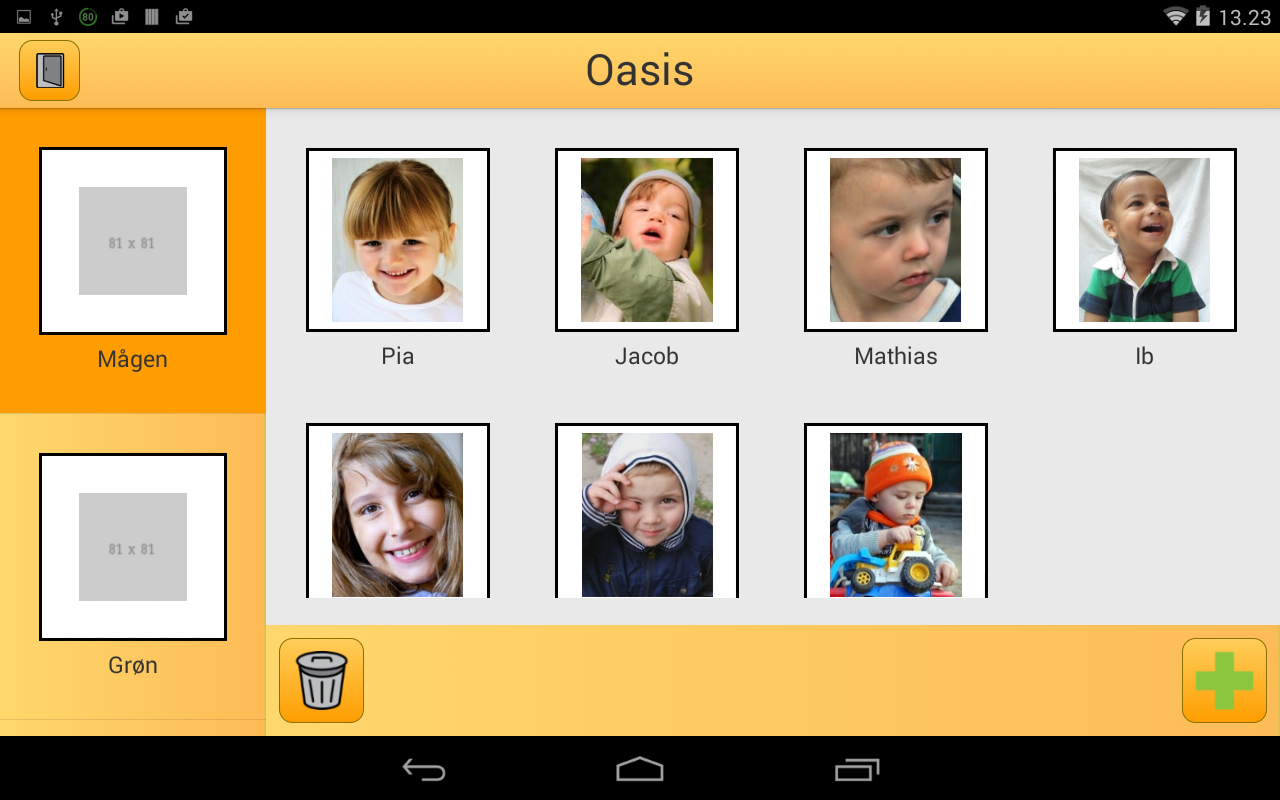
\includegraphics[width=\textwidth]{sprint_three/pictogram_component_use}
	\caption{Usage of pictogram component}
	\label{fig:pictogram_component_use}
\end{figure}